\documentclass[tikz,border=10pt]{standalone}
\usepackage{tikz}
\usetikzlibrary{patterns}

\begin{document}
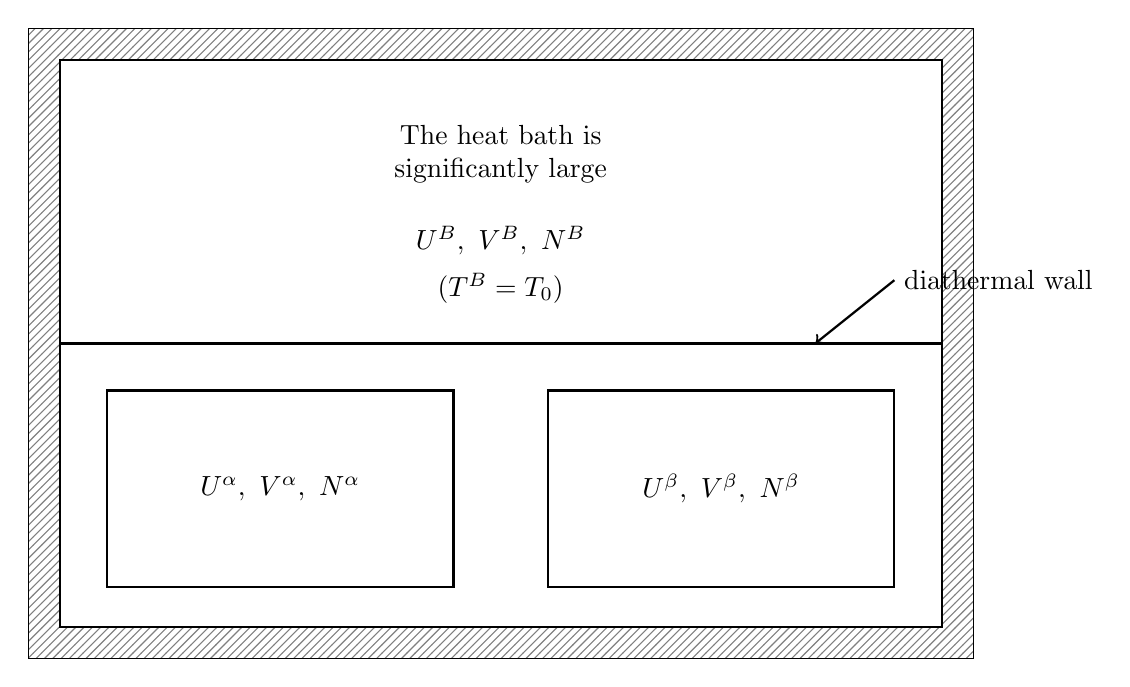
\begin{tikzpicture}
    % Outer insulated boundary
    \draw[pattern=north east lines, pattern color=black!50] (0,0) rectangle (12,8);
    \fill[white] (0.4,0.4) rectangle (11.6,7.6);
    \draw[thick] (0.4,0.4) rectangle (11.6,7.6);

    % Diathermal wall
    \draw[very thick] (0.4,4.0) -- (11.6,4.0);
    \draw[->, thick] (11.0,4.8) -- (10.0,4.0);
    \node[anchor=west] at (11.0,4.8) {diathermal wall};

    % Heat bath text
    \node[align=center] at (6.0,6.4) {The heat bath is\\significantly large};
    \node at (6.0,5.3) {$U^B,\ V^B,\ N^B$};
    \node at (6.0,4.7) {$(T^B=T_0)$};

    % Bottom subsystems
    \draw[thick] (1.0,0.9) rectangle (5.4,3.4);
    \draw[thick] (6.6,0.9) rectangle (11.0,3.4);

    \node at (3.2,2.15) {$U^\alpha,\ V^\alpha,\ N^\alpha$};
    \node at (8.8,2.15) {$U^\beta,\ V^\beta,\ N^\beta$};
\end{tikzpicture}
\end{document}
